%-----------------------------------------------------------------
% Rodrigo Chang, 2019
% Banco de Guatemala
% Programa de Estudios Superiores 2019-2020
% Diapositivas del curso "Programación I"
%
% Descargo de responsabilidad.
%   El contenido de este documento es responsabilidad exclusiva de
% su(s) autores. Cualquier opinión expresada no necesariamente
% representa la postura institucional del Banco de Guatemala. 
% 
% Contenido.
%   El contenido de estas diapositivas está construido a partir de 
% modificaciones al material provisto por Ana Bell, Eric Grimson y 
% John Guttag para el curso 6.0001 Introduction to Computer Science 
% and Programming in Python, otoño 2016, Massachusetts Institute of 
% Technology: MIT OpenCourseWare, https://ocw.mit.edu
%
% Licencia: 
% Creative Commons BY-NC-SA
% https://creativecommons.org/licenses/by-nc-sa/4.0/.
%
% Formato. 
%   El formato utilizado para la elaboración de este documento 
% ha sido modificado a partir del repositorio: 
%       https://github.com/rinnert/statlearning-python-pwf
%
% Kurt Rinnert, 2019
%   Copying and distribution of this file, with or without 
% modification, are permitted in any medium without royalty provided 
% the copyright notice and this notice are preserved. This file is 
% offered as-is, without any warranty.
%
%-----------------------------------------------------------------
\documentclass[mathserif]{beamer}
% Para configurar las diapositivas en relación 16:9, 
% agregar la opción aspectratio=169

% Título de la presentación y tópicos a tratar
\usepackage{arev, arevmath}
\usepackage[scaled]{cabin}
%\usepackage[T1]{fontenc}
\usepackage[super]{nth}
\usepackage{pifont}
\usepackage{wasysym}
\usepackage{tabularx}
\usepackage{array}
\usepackage{booktabs}
\usepackage{boldline}
\usepackage{colortbl}
\usepackage{amsmath}
\usepackage{bm}
\usepackage{tcolorbox}
\usepackage{adjustbox}
\usepackage{minibox}
\usepackage{makecell}
\usepackage{adjustbox}
\usepackage{textcomp}
\usepackage[absolute,overlay]{textpos}
\setlength{\TPHorizModule}{1mm}%
\setlength{\TPVertModule}{1mm}%
\tcbuselibrary{skins}
\usepackage{graphicx}
\usepackage[spanish, es-tabla]{babel}
\usepackage[utf8]{inputenc}
\usepackage{csquotes}

\usepackage{comment}
\usepackage{svg}

\usepackage{verbatim}
\usepackage{pdfpages}

% Columnas múltiples
\usepackage{multicol}

% -------------------------------------------
%	LISTINGS
% -------------------------------------------
% Paquetes necesarios para los códigos
\usepackage{listings}
\usepackage{color}
% Configuración de listings (pendiente)
%\input{conf/listingStyles}
% Redefinición de titulos de caption
\renewcommand\lstlistingname{\textbf{Código}}
\renewcommand\lstlistlistingname{Códigos}

% Definición de colores para Python (Jupyter notebooks)
\definecolor{python_keyword_color}{RGB}{0, 128, 0}
\definecolor{python_string_color}{RGB}{186, 34, 34}
\definecolor{python_comment_color}{RGB}{1, 121, 121}
\definecolor{frame_numbers_color}{rgb}{0.5,0.5,0.5}
\definecolor{python_identifier_color}{RGB}{0,0,0}
\definecolor{jupyter_background}{RGB}{247, 247, 247}
\definecolor{jupyter_frame}{RGB}{207, 207, 207}

% Definicion de estilo para Python
\lstdefinestyle{custom_python}{
	language=python,			% the language of the code
	backgroundcolor=\color{jupyter_background}, 
	% the size of the fonts that are used for the code
	basicstyle=\linespread{1}\small\ttfamily,	
	% Configuración de colores
	commentstyle=\color{python_comment_color},	% comment style
	identifierstyle=\color{python_identifier_color},
	keywordstyle=\mdseries\color{python_keyword_color},	% keyword style
	numberstyle=\tiny\color{frame_numbers_color},	
	stringstyle=\color{python_string_color}, % string literal style 
	captionpos=t,				% sets the caption-position to bottom
	breakatwhitespace=false,	% sets if automatic breaks should only happen at whitespace
	breaklines=true,			% sets automatic line breaking
	morekeywords={},			% if you want to add more keywords to the set
	deletekeywords={eps},		% delete keywords from the given language
	escapeinside={\%*}{*)},		% if you want to add LaTeX within your code
	framesep=3pt,
	keepspaces=true,			% keeps spaces in text,       
	numbers=none, 	% (none, left, right)
	numbersep=5pt,	% how far the line-numbers are from the code
	% if not set, the frame-color may be changed on line-breaks within not-black text (e.g. comments (green here))
	rulecolor=\color{jupyter_frame}, 
	% show spaces everywhere adding particular underscores; it overrides 'showstringspaces'
	showspaces=false,                
	% underline spaces within strings only
	showstringspaces=false,          
	% show tabs within strings adding particular underscores
	showtabs=false,                  
	stepnumber=0,	% the step between two line-numbers      
	% sets default tabsize to 2 spaces
	tabsize=2,                       
	% lets you use non-ASCII characters; for 8-bits encodings only, does not work with UTF-8
	extendedchars=true,      
	% Support additional characters            
	literate=
  {á}{{\'a}}1 {é}{{\'e}}1 {í}{{\'i}}1 {ó}{{\'o}}1 {ú}{{\'u}}1
  {Á}{{\'A}}1 {É}{{\'E}}1 {Í}{{\'I}}1 {Ó}{{\'O}}1 {Ú}{{\'U}}1
  {à}{{\`a}}1 {è}{{\`e}}1 {ì}{{\`i}}1 {ò}{{\`o}}1 {ù}{{\`u}}1
  {À}{{\`A}}1 {È}{{\'E}}1 {Ì}{{\`I}}1 {Ò}{{\`O}}1 {Ù}{{\`U}}1
  {ä}{{\"a}}1 {ë}{{\"e}}1 {ï}{{\"i}}1 {ö}{{\"o}}1 {ü}{{\"u}}1
  {Ä}{{\"A}}1 {Ë}{{\"E}}1 {Ï}{{\"I}}1 {Ö}{{\"O}}1 {Ü}{{\"U}}1
  {â}{{\^a}}1 {ê}{{\^e}}1 {î}{{\^i}}1 {ô}{{\^o}}1 {û}{{\^u}}1
  {Â}{{\^A}}1 {Ê}{{\^E}}1 {Î}{{\^I}}1 {Ô}{{\^O}}1 {Û}{{\^U}}1
  {œ}{{\oe}}1 {Œ}{{\OE}}1 {æ}{{\ae}}1 {Æ}{{\AE}}1 {ß}{{\ss}}1
  {ű}{{\H{u}}}1 {Ű}{{\H{U}}}1 {ő}{{\H{o}}}1 {Ő}{{\H{O}}}1
  {ç}{{\c c}}1 {Ç}{{\c C}}1 {ø}{{\o}}1 {å}{{\r a}}1 {Å}{{\r A}}1
  {€}{{\EUR}}1 {£}{{\pounds}}1,   
}

% Configurar el listing para el documento actual
\lstset{
	style = custom_python, 
	frame = single
}

% -------------------------------------------
%	OTRAS CONFIGURACIONES
% -------------------------------------------
\makeatletter
\newcommand{\antsize}{\@setfontsize{\antsize}{4pt}{4pt}}
\makeatother
\newcommand{\at}{\makeatletter @\makeatother}

\newcommand{\cmark}{\ding{51}}%
\newcommand{\bottomline}[1]{\vskip0pt plus 1fill{\alert{#1}\phantom{g}\vskip 1.0mm}}

% Rutas para las imágenes
%\graphicspath{{figs/}{figs/common/}}

% Separación de filas en las tablas más amplia
\renewcommand{\arraystretch}{1.2}


% -------------------------------------------
%	ESTILO DE LA PRESENTACIÓN
% -------------------------------------------

\mode<presentation>%
{
	\usetheme{default}
	%\usetheme[width=2.5cm]{PaloAlto}
	\usecolortheme{dove}
	\useoutertheme{infolines}
	% oder auch nicht

	% BANGUAT Colors
	\definecolor{BANGUATblue}{RGB}{37,86,162} % 0x255682
	\definecolor{BANGUATorange}{RGB}{255,130,0} % 0xff8200
	\definecolor{BANGUATgreen}{RGB}{0,100,0}
	\definecolor{BANGUATdark}{RGB}{80,80,80} % 0x505050
	\definecolor{BANGUATlight}{RGB}{120,120,120}
	\definecolor{BANGUATbrown}{RGB}{178,91,0}

	\definecolor{codebg}{rgb}{0.95,0.95,0.95}

	% Color theme
	\setbeamercolor{alerted text}{fg=BANGUATorange}
	\setbeamercolor{frametitle}{fg=BANGUATblue}
	\setbeamercolor{title}{fg=BANGUATblue}
	\setbeamercolor{subtitle}{fg=BANGUATorange}
	\setbeamercolor{normal text}{fg=BANGUATdark}
	\setbeamercolor{author in foot}{fg=BANGUATblue}
	\setbeamercolor{item}{fg=BANGUATblue}
	\setbeamercolor{footline}{fg=BANGUATblue}
	%\setbeamercolor{item projected}{bg=BANGUATorange}
	%\setbeamercolor{item projected}{fg=white}

	\setbeamertemplate{headline}
	{}
	\setbeamertemplate{frametitle}
	{
		%\textbf{{\insertframetitle\phantom{g}}}\\
		%\textbf{\insertframetitle\phantom{g}}\\
		\textbf{\underline{\insertframetitle\phantom{g}}}\\
		%\textbf{\underline{\insertframetitle}}\\
		\vskip 1.0mm
		%{\color{UOLgold}\hrule height 2pt}
		%\par
	}
	\addtobeamertemplate{frametitle}{}{\vspace{-1em}}
	\setbeamertemplate{footline}{
		{%
			\textbf{ \hskip 3.0mm\insertshorttitle\phantom{.}---\phantom{.}\insertshortinstitute\hfill\insertframenumber\,/\,\inserttotalframenumber\hskip 3.0mm} 
		}
	}

	\setbeamertemplate{navigation symbols}{}%remove navigation symbols
	\setbeamertemplate{itemize items}[circle]
	\setbeamertemplate{enumerate items}[fg=BANGUATblue]
	\setbeamercolor{itemize items}{fg=BANGUATblue}
	\setbeamercolor{sidebar}{bg=BANGUATblue}
	\setbeamercolor{title in sidebar}{fg=BANGUATorange}
	\setbeamercolor{author in sidebar}{fg=BANGUATorange}
	\setbeamercolor{section in sidebar}{fg=BANGUATorange}
}



% -------------------------------------------
%	CONFIGURACIÓN DE DIAPOSITIVA DE TÍTULO
% -------------------------------------------

% Título del curso
\title[Programación I]{\textbf{%
Introducción a las ciencias de la computación\\%
{\it y programación en Python}}\\%
%\href{https://ocw.mit.edu/courses/electrical-engineering-and-computer-science/6-0001-introduction-to-computer-science-and-programming-in-python-fall-2016/}{\tiny\it Basado en el curso ``Introduction to Computer Science and Programming in Python'' por Ana Bell, Eric Grimson, y John Guttag.}%
\vspace{3em}%
}
%\vspace{-2.5cm}{}

% Autor y correo electrónico
\author{\href{mailto:?to=Rodrigo Chang <rrcp@banguat.gob.gt>&subject=PES Programación I}{Rodrigo Chang}}

% Información del instituto
\institute[\href{https://www.banguat.gob.gt/}{Banco de Guatemala}]%
{\color{BANGUATblue} \bfseries \href{https://www.banguat.gob.gt/}{Banco de Guatemala}\\%
\vspace{3mm}%

\includegraphics[width=0.13\textwidth]{figs/common/logo-banguat.png}}

% Sin fecha en particular
\date{}

% Información de licencias y copyright
\titlegraphic{
	 %\texorpdfstring{\vspace{-3cm}}{}
	 \vspace{-1.5cm}
	 \begin{minipage}[b][1cm][b]{0.25\textwidth}%
	    \color{BANGUATlight}\antsize
		%Copyright \textcopyright~2019\\
		\href{mailto:?to=Rodrigo Chang <rrcp@banguat.gob.gt>&subject=PES Programación I}{Rodrigo Chang <rrcp@banguat.gob.gt>}\\
		Este material está construido a partir de modificaciones al material provisto por Ana Bell, Eric Grimson y John Guttag para el curso \textit{6.0001 Introduction to Computer Science and Programming in Python}, otoño 2016, Massachusetts Institute of Technology: MIT OpenCourseWare, \href{https://ocw.mit.edu}{https://ocw.mit.edu}. Licencia: \href{https://creativecommons.org/licenses/by-nc-sa/4.0/}{Creative Commons BY-NC-SA}.
		
		%Copying and distribution of this file, with or without modification, are permitted in any medium without royalty provided the copyright notice and this notice are preserved.  This file is offered as-is, without any warranty.


		%Some of the figures in this presentation are taken from ``An Introduction to Statistical Learning, with applications in R''  (Springer, 2013) with permission from the authors: G. James, D. Witten,  T. Hastie and R. Tibshirani 
	 \end{minipage}%
	 \hspace{9cm}
}

% Restar uno al contador
\addtocounter{framenumber}{-1}

% Cajas de colores
\newcommand{\tabboxset}{\tcbset{enhanced, nobeforeafter, boxrule=0pt, boxsep=0pt, colback=codebg, colframe=codebg, coltext=BANGUATdark, rounded corners, arc=4pt, fonttitle={\bfseries\tiny}}}
\newcommand{\codeboxset}{\tcbset{enhanced, nobeforeafter, boxrule=0pt, boxsep=0pt, colback=codebg, colframe=codebg, coltext=BANGUATdark, rounded corners, arc=4pt, fonttitle={\bfseries\tiny}}}

% Comandos útiles
\newcommand{\orange}{\color{BANGUATorange}}
\newcommand{\blue}{\color{BANGUATblue}}
\newcommand{\dark}{\color{BANGUATdark}}
\newcommand{\R}{\mathbb{R}}
\newcommand{\dat}[1]{{\footnotesize\tt\orange #1}}
\newcommand{\mdat}[1]{\text{\dat{#1}}}
\newcommand{\val}[1]{{\footnotesize\tt\blue #1}}
\newcommand{\mval}[1]{\text{\val{#1}}}
\newcommand{\e}[1]{\emph{#1}}
\newcommand{\bh}{\hat{\beta}}
\newcommand{\h}{\hat}
\newcommand{\bl}{\bottomline}


\makeatletter
\newcommand{\includegraphicsdpi}[3]{%
	\pdfimageresolution=#1%
	\includegraphics[#2]{#3}%
	\pdfimageresolution=72%
}

\newcommand{\Quote}[2]{%
	\begin{center} 
		\begin{minipage}{0.7\textwidth} 
			\hrule
			\vskip 3mm
			\emph{{\color{BANGUATblue} ``#1''}\\
			{\color{BANGUATorange} --- #2}}
			\vskip 3mm
			\hrule
			\vskip 2mm
		\end{minipage}
	\end{center}
}

% Texto centrado en la diapositiva, quizás para el abstract o para indicar abajo de un quote
\newenvironment{blurb}%
	{\begin{center}\begin{minipage}{0.6\textwidth}\footnotesize}
	{\end{minipage}\end{center}}

% Environment para códigos o algoritmos. Parecido a un bottomline, se puede utilizar para dar definiciones o enfatizar en algún concepto
\newenvironment{cpage}%
	{\begin{center}\begin{minipage}{0.75\textwidth}}
	{\end{minipage}\end{center}}

% Bloque (similar a un pop-up) de alerta para indicar resultados en tablas, definiciones, fórmulas, etc.
% Primer argumento es el tamaño 
% Segundo argumento es el título del bloque
\newenvironment{popblock}[2]%
	{\begin{center}\begin{minipage}{#1}\footnotesize
		\begin{tcolorbox}[colframe=codebg, colback=white, colupper=BANGUATdark, title={\normalsize\bfseries\blue #2}]}
	{\end{tcolorbox}\end{minipage}\end{center}}
\makeatother

% Incluir diapositivas en PDF
% 1 - Título de la diapositiva
% 2 - páginas del PDF a incluir
% 3 - ruta hacia el archivo PDF
\newcommand{\includeslides}[3]{%
{%
\setbeamercolor{background canvas}{bg=}%
\addtocounter{framenumber}{1}%
\includepdf[pages={#1}, link=true, pagecommand={%
\Large\blue\bfseries\underline{%
#3\phantom{g}}%
\vspace{-1em}%
\vskip 1.0mm}]{#2}%
}}
\subtitle{%
  \bfseries{Funciones: descomposición y abstracción}\\%
  %{\tiny\it Manejo de strings, \textit{guess and check}, métodos de aproximación}\\%
}

% Inicio del documento
\begin{document}
\frame[plain]{
	%\vskip 1.0mm
	\titlepage
	%\vskip 1.0mm
}
%-----------------------------------------------------------------
% Empieza el contenido de la presentación
%-----------------------------------------------------------------

\begin{frame}{Abstract}
	\Quote{Programs must be written for people to read, and only incidentally for machines to execute.}{Harold Abelson, Structure and Interpretation of Computer Programs }
    
	\begin{blurb}
		Veremos cómo estructurar programas en funciones para ocultar detalles.
		
		Hablaremos de los conceptos de alcance (\textit{scope}) y espacio de nombres (\textit{name space}) en Python.
		
	\end{blurb}
\end{frame}

\section{Descomposición y abstracción}

\begin{frame}[fragile]{¿Cómo escribimos código?}
    \begin{itemize}
        \item Hasta ahora: 
        \begin{itemize}
            \item Hemos visto algunos mecanismos del lenguaje.
            \item Código en un bloque (celda) representa algún cómputo.
            \item Cada archivo (celda) es una pieza de código.
            \begin{itemize}
                \item Cada código es una secuencia de instrucciones.
            \end{itemize}
        \end{itemize}
        
        \item Algunos {\blue problemas}:
        \begin{itemize}
            \item Es fácil para problemas a \textit{pequeña escala}.
            \item Es {\blue\bfseries muy desordenado} para problemas más grandes.
            
            \item Es difícil {\blue\bfseries seguir} los detalles.
            \item Información correcta $\Rightarrow$ parte código del código.
        \end{itemize}
    \end{itemize}
\end{frame}

\begin{frame}{Buenas prácticas}
    \begin{itemize}
        \item Más código {\orange\bfseries no} es necesariamente algo bueno.
        
        \item Cantidad de \textit{funcionalidad} $\Rightarrow$ buenos programadores.
        
        \item Necesitamos un mecanismo para {\blue\bfseries descomponer} el código y {\blue\bfseries abstraer} la funcionalidad.
        
        \item Para esto, introducimos las {\bfseries\orange funciones}.
    \end{itemize}
\end{frame}

\begin{frame}[fragile]{Abstracción}
    \begin{itemize}
        \item Un proyector es una caja negra --- {\blue no sabemos cómo funciona}. 
        \item Sabemos cómo se utiliza y para qué sirve.
        \item Conocemos la entrada: cualquier dispositivo electrónico que se pueda conectar.
        \item Y la salida que produce.
        \item Es una caja negra que convierte y magnifica imágenes de la entrada hacia una pantalla (pared).
        
    \end{itemize}
    \bottomline{Esta es la idea detrás de la abstracción: no necesitamos saber cómo funciona para utilizarlo.}
\end{frame}

\begin{frame}[fragile]{Descomposición}
    \begin{itemize}
        \item Supongamos que queremos proyectar imágenes para las Olimpiadas con varios proyectores.
        \item Cada proyector recibe una entrada y produce una salida individual.
        \item Todos producen una imagen más grande.
        
    \end{itemize}
    \bottomline{Esta es la idea detrás de la descomposición: diferentes dispositivos trabajan en conjunto para lograr un objetivo.}
\end{frame}

\begin{frame}[fragile]{Crear estructura con la descomposición}
    \begin{itemize}
        \item En programación, el código se divide en {\blue\bfseries módulos}:
        \begin{itemize}
            \item {\orange autocontenidos}
            \item permiten {\orange\bfseries separar} el código,
            \item {\orange\bfseries reutilizarlo},
            \item mantenerlo {\orange\bfseries organizado} y 
            \item {\bfseries\orange coherente}.
        \end{itemize}
    \end{itemize}
    
    \bottomline{Ahora utilizaremos funciones para descomponer el código, más adelante utilizaremos clases.}
\end{frame}

\begin{frame}[fragile]{Omitir detalles con la abstracción}
    \begin{itemize}
        \item En programación, puede pensarse en una {\blue\bfseries caja negra}: 
        \begin{itemize}
            \item No se quieren/necesitan ver los detalles.
            \item Esconder detalles tediosos en el código.
        \end{itemize}
        
        \item Esto lo lograremos con la {\bfseries\blue especificación adecuada} de una función:
        \begin{itemize}
            \item ¿Qué recibe como entradas y qué devuelve como salidas?.
        \end{itemize}
        
        \item También será útil definir un {\blue\bfseries docstring}.
    \end{itemize}
    
    \bottomline{Ahora utilizaremos funciones para descomponer el código, más adelante utilizaremos clases.}
\end{frame}

\begin{frame}[fragile]{Funciones}
    \begin{itemize}
        \item {\blue\bfseries Piezas} de código reutilizables.
        
        \item No se ejecutan hasta ser {\orange\bfseries llamadas} o {\orange\bfseries ``invocadas''}.
        
        \item Características: 
        \begin{itemize}
            \item Nombre
            \item Parámetros (0 o más)
            \item {\blue docstring}
            \item cuerpo
            \item {\blue devuelven} un resultado
        \end{itemize}
    \end{itemize}
\end{frame}

\begin{frame}[fragile]{Ejemplo}
    \begin{itemize}
        \item Veamos una función sencilla
    \end{itemize}
\begin{lstlisting}
# Def. de funcion par
def esPar(i):
    """ 
    Input: i, entero positivo
    Devuelve True si i es par, si no, False
    """
    remainder = i % 2
    return remainder == 0
\end{lstlisting}
\end{frame}



\section{Alcance (\textit scope) de las variables}

\begin{frame}[fragile]{Alcance (\textit scope) de las variables}
    \begin{itemize}
        \item Una función crea un nuevo ambiente/marco/\textit{scope} {\blue\bfseries cuando se ejecuta}.
        
        \item {\blue\bfseries scope} se refiere al mapeo de nombres a objetos.
        
        \item El {\orange parámetro formal} recibe el valor del {\orange parámetro real}.  
    
\begin{lstlisting}
def f(x):
    x = x + 1
    print('dentro de f(x): x =', x)
    return x

x = 3
z = f( x )
\end{lstlisting}
        
        \item \href{http://www.pythontutor.com/visualize.html#code=def%20f%28x%29%3A%0A%20%20%20%20x%20%3D%20x%20%2B%201%0A%20%20%20%20print%28'in%20f%28x%29%3A%20x%20%3D',%20x%29%0A%20%20%20%20return%20x%0A%0Ax%20%3D%203%0Az%20%3D%20f%28%20x%20%3D%20x%20%29&cumulative=false&curInstr=0&heapPrimitives=nevernest&mode=display&origin=opt-frontend.js&py=3&rawInputLstJSON=%5B%5D&textReferences=false}{Ver en Python Tutor}
    
    \end{itemize}
    \bottomline{¿Qué pasa si \lstinline|z = f( x = x )|? }
\end{frame}


\begin{frame}[fragile]{Funciones sin \lstinline|return|}
    \begin{itemize}
        \item También llamadas {\blue procedimientos}. 
        \item En Python, devuelven \lstinline|None| (ausencia de valor).
    \end{itemize}
\begin{lstlisting}
# Def. de funcion par
def esPar(i):
    """ 
    Input: i, entero positivo
    Imprime True si i es par, si no, False
    """
    remainder = i % 2
    print(remainder == 0)
\end{lstlisting}
\end{frame}

% Diferencia print vs return
\begin{frame}[fragile]{\lstinline|return| vs. \lstinline|print|}
    \begin{columns}
        \begin{column}{0.5\textwidth}
        \lstinline|return|:
        \begin{itemize}
            \item Significado {\blue dentro} de una función.
            \item Se ejecuta {\blue\bfseries solo uno}.
            \item Después de \lstinline|return|, código es {\blue ignorado}.
            \item Tiene valor asociado, {\blue devuelto a quién invoca la función}.
        \end{itemize}
        \end{column}
        \begin{column}{0.5\textwidth}
        \begin{itemize}
            \item Puede ser utilizado {\blue fuera} de una función.
            \item Pueden ejecutarse {\blue\bfseries varios}.
            \item Después de \lstinline|print|, código es {\blue ejecutado}.
            \item Devuelve \lstinline|None|, pero su salida es hacia la {\blue\bfseries consola}.
        \end{itemize}
        \end{column}
    \end{columns}
\end{frame}

% Funciones pueden ser argumentos y valores de retorno
\includeslides{21-24}{slides-60001/MIT6_0001F16_Lec4_mod.pdf}{Funciones como argumentos}

% Ejemplo de scopes

\begin{frame}[fragile]{Scope (ambiente/alcance)}
    \begin{itemize}
        \item Dentro de una función, {\blue\bfseries se puede acceder} a una variable definida afuera.     
\begin{lstlisting}
def g(y):
    print(x)
    print(x+y)

x = 5
g(x)
print(x)
\end{lstlisting}

    \item Otro ejemplo: 
\begin{lstlisting}
def g(y):
    print(x)

x = 5
g(x)
print(x)
\end{lstlisting}
        
    \end{itemize}
\end{frame}

\begin{frame}[fragile]{Scope (ambiente/alcance)}
    \begin{itemize}
        \item Dentro de una función, {\blue\bfseries no se puede modificar una variable\footnote{Excepto si la variable es mutable} definida afuera.}
\begin{lstlisting}
def h(y):
    x += 1

x = 5
h(x)
print(x)
\end{lstlisting}
    
    \item \href{https://www.python-course.eu/python3_passing_arguments.php}{¿Cómo funcionan los argumentos en Python?}
    
    \end{itemize}
\end{frame}

\begin{frame}[fragile]{Detalles en el \textit{scope}}
    \begin{itemize}
        \item Veamos un ejemplo más detallado: 
\begin{lstlisting}
def g(x):
    def h():
        x = 'abc'
    x = x + 1
    print('in g(x): x =', x)
    h()
    return x

x = 3
z = g(x)
\end{lstlisting}
        
        \item \href{http://www.pythontutor.com/visualize.html#code=def%20g(x%29%3A%0A%20%20%20%20def%20h(%29%3A%0A%20%20%20%20%20%20%20%20x%20%3D%20'abc'%0A%20%20%20%20x%20%3D%20x%20%2B%201%0A%20%20%20%20print('in%20g(x%29%3A%20x%20%3D',%20x%29%0A%20%20%20%20h(%29%0A%20%20%20%20return%20x%0A%0Ax%20%3D%203%0Az%20%3D%20g(x%29&cumulative=false&curInstr=0&heapPrimitives=false&mode=display&origin=opt-frontend.js&py=3&rawInputLstJSON=%5B%5D&textReferences=false}{Ver en Python Tutor}
    \end{itemize}
\end{frame}

% Ejecución del ejemplo anterior 
\includeslides{29-33}{slides-60001/MIT6_0001F16_Lec4_mod.pdf}{Detalles en el \textit{scope}}

\begin{frame}[fragile]{Descomposición y abstracción}
    \begin{itemize}
        \item Concepto {\blue\bfseries poderoso}.
        
        \item El código es {\blue\bfseries REUTILIZABLE} y solamente tiene que ser {\orange\bfseries depurado} una vez.
    \end{itemize}
\end{frame}

% Paso de argumentos
% https://www.python-course.eu/python3_passing_arguments.php

%-----------------------------------------------------------------
% Termina el contenido de la presentación
%-----------------------------------------------------------------

\begin{comment}

% Slide with two columns, half and half
\begin{frame}[fragile]{}
    \begin{columns}
        \begin{column}{0.5\textwidth}
        \end{column}
        \begin{column}{0.5\textwidth}
        \end{column}
    \end{columns}
\end{frame}

% Slide with bullets
\begin{frame}[fragile]{}
    \begin{itemize}
        \item 
    \end{itemize}
\end{frame}

% Slide with bullets and code
\begin{frame}[fragile]{}
    \begin{itemize}
        \item 
    \end{itemize}
\begin{lstlisting}
Code goes here
\end{lstlisting}
\end{frame}

% Include PDF 
\setbeamercolor{background canvas}{bg=}
\includepdf[pages=541-542, link=true, fitpaper]{slides-60001/MIT6_0001F16_Lec4.pdf}

% Include PDF slides with title
\setbeamercolor{background canvas}{bg=}
\includepdf[pages={21-22}, link=true, pagecommand={%
\Large\blue\bfseries\underline{%
Título de las diapositivas\phantom{g}}%
\vspace{-1em}%
\vskip 1.0mm}]{slides-60001/MIT6_0001F16_Lec4_mod.pdf}

% Pytutor
\href{URL}{Ver en Python Tutor}


\end{comment}

\end{document}